\section{Introduction}
\label{sec:introduction}

Reinforcement learning (RL) describes the sequential decision-making process where an agent interacts with the environment to maximize the cumulative reward signal \cite{sutton1999reinforcement}. With the development of deep learning, deep reinforcement learning (DRL) has emerged as a powerful paradigm that combines deep neural networks with traditional reinforcement learning algorithms, making it possible to learn complex behavior representations from high-dimensional sensory inputs \cite{li2017deep}. Such paradigm empowers the agent to learn effective behavior policies in various real-world scenarios such as robotics control \cite{kober2013reinforcement}, game playing \cite{silver2018general}, and autonomous driving \cite{kiran2021deep}.

In the traditonal setting, the agent learns in an online manner, which requires the agent to frequently interact with the environment to gather samples. However, such interaction can be extremely expensive in some real-world applications. On one hand, collecting real-world samples can hardly be parallelized, which makes the process remarkably slow. On the other hand, the agent may suffer from catastrophic failures during the learning process, which may not be affordable in safety-critical applications. To address these issues, researchers have proposed an alternative offline manner, where the agent learns from a fixed dataset without interacting with the environment \cite{levine2020offline} as shown in Figure \ref{fig:offline_rl}. Admittedly, the offline reinforcement learning paradigm is attractive, but it also faces several challenges. The bootstrap method unavoidably introduces distribution shifts, which makes the traditional algorithms fail to learn a satisfactory policy. Researchers have proposed various methods to tackle this problem, such as implicit Q-learning \cite{kostrikov2021offline}, conservative Q-learning \cite{kumar2020conservative}, and TD3-BC \cite{fujimoto2021minimalist}. The core idea of these methods is to suppress the overestimation of the Q-value function, which is widely recognized as the main reason for the failure of offline reinforcement learning.

\begin{figure}[ht]
    \centering
    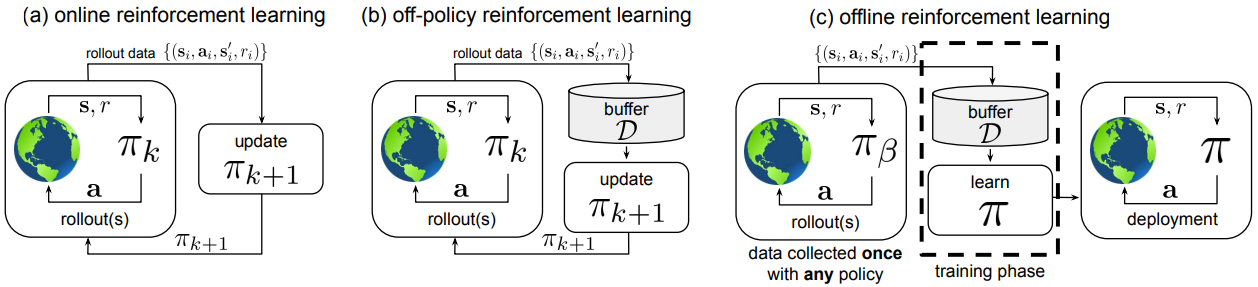
\includegraphics[width=0.9\textwidth]{figure/offline_rl.png}
    \caption{An illustration of online reinforcement learning, off-policy reinforcement learning, and offline reinforcement learning. Offline reinforcement learning follows an open-loop control paradigm, where the agent learns from a fixed dataset without interacting with the environment.}
    \label{fig:offline_rl}
\end{figure}

When it comes to scaling up the reinforcement learning algorithms, researchers find that learning multiple tasks simultaneously can effectively improve the sample efficiency and generalization ability of the agent as shown in Figure \ref{fig:multi_task}. Multi-task reinforcement learning (MTRL) thus becomes a popular research direction in recent years \cite{vithayathil2020survey}. Researchers have proposed various methods for the multi-task setting, including shared representation learning \cite{borsa2016learning}, knowledge transfer and distillation \cite{xu2020knowledge}, and progressive neural networks \cite{rusu2016progressive}. However, most of these methods are designed for the online setting, so they will suffer from the same issues when applied to the offline setting. Some novel methods have been proposed to combine the offline and multi-task learning paradigms, such as conservative data sharing \cite{yu2021conservative} and scaled Q-learning \cite{kumar2022offline}, but how to achieve reliable offline multi-task reinforcement learning still remains an open problem till today.

\begin{figure}[ht]
    \centering
    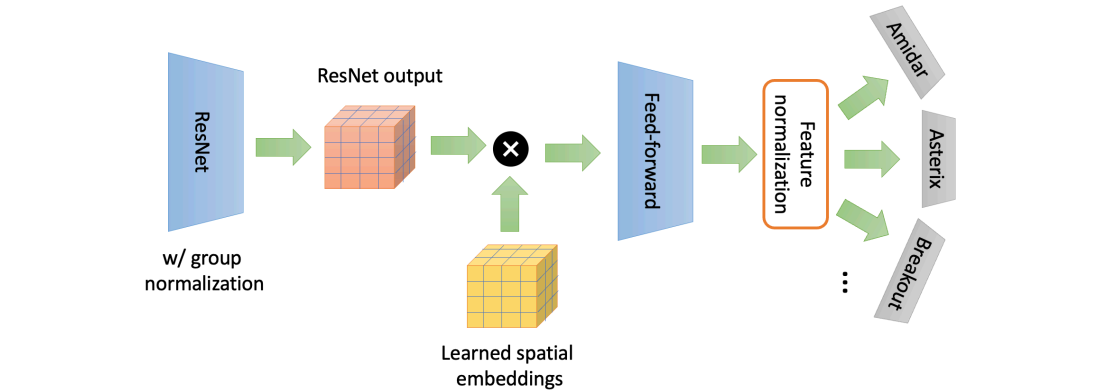
\includegraphics[width=0.9\textwidth]{figure/multi_task.png}
    \caption{An example of multi-task reinforcement learning. Multiple policy heads share the same backbone as the feature extractor to learn useful shared representations, so that the agent can benefit from the extensive experience and knowledge transfer across multiple tasks.}
    \label{fig:multi_task}
\end{figure}

In this project, we aim to explore the offline multi-task reinforcement learning paradigm. Our study pivots around improving the sample efficiency and generalization ability of the agent by fully exploiting the potential of multi-task learning. We propose a novel algorithm framework named heuristic conservative soft actor-critic (HCSAC) to solve the offline multi-task reinforcement learning problem. The framework is built upon the conservative Q-learning \cite{kumar2020conservative} and soft actor-critic \cite{haarnoja2018soft} algorithms to suppress distribution shifts in the offline setting. We also introduce task embeddings to allow the agent to learn shared representations across multiple tasks. In addition, we follow conservative data sharing \cite{yu2021conservative} and propose a heuristic strategy to relabel the dataset, so that the agent can benefit from the augmented transitions while avoiding performance degradation. We conduct a series of experiments on the MuJoCo benchmark \cite{todorov2012mujoco} to evaluate the performance of our method. Through these efforts, we expect to provide some insights into the characteristics and efficacies of the proposed method, and to demonstrate the potential of offline multi-task reinforcement learning in real-world applications.